\section{Code completion with NLMs}
Language modelling faces a difficult problem when it comes to code completion. There are local (to only one block of code) and very long distance dependencies in coding, such as initializing a variable only once per function. One approach involved merging a model employing pointer networks with attention, which was shown to perform better at simulating long distance dependencies than RNNs and LSTMs~\cite{ccnlm}.

\subsection{Pointer Networks (Ptr-Net)}
Pointer networks~\cite{pointer} are built on top of modified attention mechanism with pointers to input words. Figure~\ref{fig:1b} illustrates these pointers.

\begin{figure}[hbt!]
\centering 
\subfloat[Sequence-to-Sequence.\label{fig:1a}]{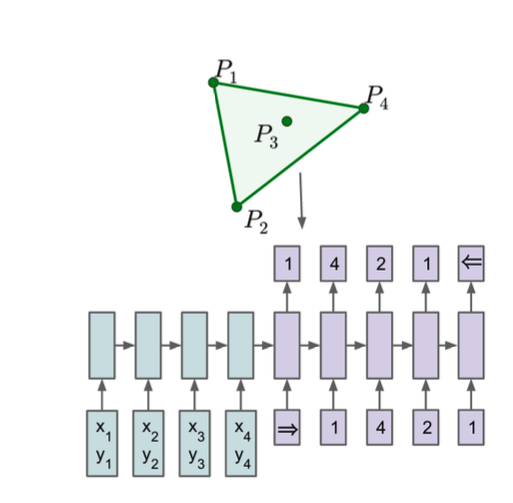
\includegraphics[width=0.5\textwidth]{Figures/seq.png}}\hfill
\subfloat[Ptr-Net.\label{fig:1b}] {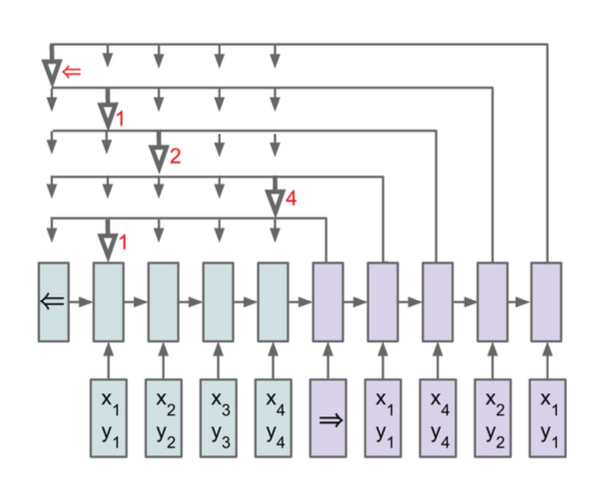
\includegraphics[width=0.5\textwidth]{Figures/soft_max.png}}
\caption{Comparison of a Transformer (Sequence-to-Sequence model with a Ptr-Net.)~\cite{pointer}.} 
\label{fig:pointer}
\end{figure}

By predicting words from the input sequence, Ptr-Nets offer a solution to the challenge of anticipating words that are not in one's vocabulary. However, Ptr-Nets can only anticipate words that appear in the local context because they cannot predict words outside of the input sequence (like a block of code).

Due to this restriction, the Pointer Mixture Network, which predicts words either from the global vocabulary or copies one from local context, was introduced~\cite{ccnlm}. It combines Attention (long dependencies) and Ptr-Nets (local dependencies). In addition, a modified version of the Attention mechanism using an AST-based programming language was developed in this study~\cite{ccnlm}.

\subsection{GitHub Copilot}



\subsection{Alternatives to Copilot}
There are a handful of code completion systems currently being used, below is a list a few such systems:

\begin{itemize}
    \item IntelliSense [8] - Microsoft’s implementation of a code completion / suggestion tool which is included in Jetbrains IDEs.
    \item Jedi [5] - A python static analysis tool aimed at automatic code completion in python.
    \item Kite - https://www.kite.com
    \item Deep TabNine [1] - Deep TabNine is a closed source code completion system which
was trained on GPT-2.
    \item AlphaCode - 
    \item CodeBERT -
    \item PaLM - 
\end{itemize}
